%++++++++++++++++++++++++++++++++++++++++
% Don't modify this section unless you know what you're doing!
\documentclass[letterpaper,12pt]{article}
\usepackage{tabularx} % extra features for tabular environment
\usepackage{amsmath}  % improve math presentation
\usepackage{graphicx} % takes care of graphic including machinery
\usepackage[margin=0.8in,letterpaper]{geometry} % decreases margins
\usepackage{cite} % takes care of citations
\usepackage[final]{hyperref} % adds hyper links inside the generated pdf file
\usepackage{pgfplotstable, booktabs}
\usepackage{placeins}
\usepackage{tabularray}
\usepackage{titlesec}
\usepackage{fancyhdr}
\usepackage{empheq}
\usepackage{amssymb}
\usepackage{sectsty}
\usepackage{tcolorbox}
\usepackage{listings}
\usepackage{xcolor}
\usepackage{parskip}
\usepackage{cancel}
\usepackage{enumitem}
\usepackage{mathrsfs}
\usepackage{physics}
\usepackage{subcaption}
\usepackage{pdfpages}
\usepackage{amsthm} 
\usepackage{float}
\usepackage{titlesec}
\usepackage{breqn}

% sets the number of sectioning levels that get number and appear in the contents
\titleclass{\subsubsubsection}{straight}[\subsection]

\newcounter{subsubsubsection}[subsubsection]
\renewcommand\thesubsubsubsection{\thesubsubsection.\arabic{subsubsubsection}}
\renewcommand\theparagraph{\thesubsubsubsection.\arabic{paragraph}} % optional; useful if paragraphs are to be numbered

\titleformat{\subsubsubsection}
  {\normalfont\normalsize\bfseries}{\thesubsubsubsection}{1em}{}
\titlespacing*{\subsubsubsection}
{0pt}{3.25ex plus 1ex minus .2ex}{1.5ex plus .2ex}

\makeatletter
\renewcommand\paragraph{\@startsection{paragraph}{5}{\z@}%
  {3.25ex \@plus1ex \@minus.2ex}%
  {-1em}%
  {\normalfont\normalsize\bfseries}}
\renewcommand\subparagraph{\@startsection{subparagraph}{6}{\parindent}%
  {3.25ex \@plus1ex \@minus .2ex}%
  {-1em}%
  {\normalfont\normalsize\bfseries}}
\def\toclevel@subsubsubsection{4}
\def\toclevel@paragraph{5}
\def\toclevel@paragraph{6}
\def\l@subsubsubsection{\@dottedtocline{4}{7em}{4em}}
\def\l@paragraph{\@dottedtocline{5}{10em}{5em}}
\def\l@subparagraph{\@dottedtocline{6}{14em}{6em}}
\makeatother

\setcounter{secnumdepth}{4}
\setcounter{tocdepth}{4}



\definecolor{codegreen}{rgb}{0,0.6,0}
\definecolor{codegray}{rgb}{0.5,0.5,0.5}
\definecolor{codepurple}{rgb}{0.58,0,0.82}

\lstdefinestyle{mystyle}{
    commentstyle=\color{codegreen},
    keywordstyle=\color{codepurple},
    numberstyle=\tiny\color{codegray},
    stringstyle=\color{codegreen},
    basicstyle=\ttfamily\small,
    breakatwhitespace=false,         
    breaklines=true,                 
    captionpos=b,                    
    keepspaces=true,                                                     
    showspaces=false,                
    showstringspaces=false,
    showtabs=false,                  
    tabsize=4
}

\lstset{style=mystyle}
  
\newcommand*\widefbox[1]{\fbox{\hspace{0em}#1\hspace{0em}}}
\DeclareMathOperator{\Div}{div}
\DeclareMathOperator{\Grad}{grad}
\DeclareMathOperator{\Curl}{curl}

\pagestyle{fancy}
\fancyhf{} % Clear all header and footer fields
\fancyhead[L]{MEC E 539}
%\fancyhead[C]{Center Header} 
\fancyhead[C]{Lecture Notes}
\fancyhead[R]{Alex Diep}
\setlength{\headheight}{15pt}

\fancyfoot[C]{\thepage}

\pgfplotsset{compat=1.18} 
\titleformat*{\section}{\Large\bfseries}
\titleformat*{\subsection}{\large\bfseries}

% \renewcommand{\thesection}{Question \arabic{section}}
% \renewcommand{\thesubsection}{(\alph{subsection})}
\renewcommand*{\arraystretch}{2}
\setlength{\jot}{10pt}

\hypersetup{
	colorlinks=true,       % false: boxed links; true: colored links
	linkcolor=blue,        % color of internal links
	citecolor=blue,        % color of links to bibliography
	filecolor=magenta,     % color of file links
	urlcolor=blue         
}

% Define Custom Table Column Types
\newcolumntype{C}[1]{>{\centering\arraybackslash}p{#1}}

%++++++++++++++++++++++++++++++++++++++++
\begin{document}
% \begin{titlepage}
%     \centering
%     \vspace*{2cm} % Adjust vertical spacing
    
%     % Title
%     \Huge {MEC E 301 \\Lab 1: Dimensional Measurement} \\
%     \vspace{1cm} % Adjust vertical spacing
    
%     % Author
%     \Large by: Alex Diep \\
%     \vspace{1cm} % Adjust vertical spacing

%     % Date
%     \Large Date: September 19, 2023 \\ % or manually specify a date
%     \vspace{4cm} % Adjust vertical spacing

%     % CCID and Student ID in smtaller font
%     \normalsize CCID: abdiep \\
%     \normalsize Student ID: 1664334 \\ 
%     \normalsize Section: D21 \\
    
%     \vfill % Fill vertical space
    
%     % Additional content (e.g., university logo or other information)
    
% \end{titlepage}

% TOC
\pagenumbering{gobble}
\pagenumbering{roman}
% Table of Contents (Hyperlinks set to locally black)
{
    \hypersetup{hidelinks}
    \tableofcontents
}
\newpage
{
    \hypersetup{linkcolor=black}
    \listoffigures
    \listoftables
}
\newpage
\pagenumbering{arabic}

\section{Tensor Notation}
\begin{table}[H]
    \centering
    \caption{Different Rank Tensors}
    \begin{tabular}{cccc}
        \toprule
        Rank & Name & Notation & Example \\
        \midrule
        0 & Scalar & $T$ & Temperature, Pressure, Volume \\
        1 & Vector & $T_i$ & Force, Velocity, Vorticity \\
        2 & Matrix & $T_{ij}$ & Stress, Strain, Rate of Deformation \\
        3 & Third Order Tensor & $T_{ijk}$ & ... \\
        4 & Fourth Order Tensor & $T_{ijkl}$ & ... \\
        ... & ... & ... & ... \\
        \bottomrule
    \end{tabular}
\end{table}

\subsection{Einstein Summation Convention}
The Einstein Summation Convention is a shorthand notation for writing out long sums. It is used to simplify the notation of tensor operations. The convention is as follows:
\begin{itemize}
    \item If an index appears more than once in a term, it is a dummy index. It is summed over.
    \item If an index appears once in a term, it is a free index. The number of free indices is the rank of the tensor.
\end{itemize}

\subsubsection{Examples}
\subsubsubsection{Example 1}

Consider,
\begin{align*}
    A_{ij} &=
    \begin{bmatrix}
        A_{11} & A_{12} & A_{13} \\
        A_{21} & A_{22} & A_{23} \\
        A_{31} & A_{32} & A_{33}
    \end{bmatrix} 
\end{align*}
There are two free indices, $i$ and $j$. The rank of the tensor is 2. \\

\subsubsubsection{Example 2}

Consider, 
\begin{align*}
    \partial_i u_{ij} &= \begin{bmatrix}
        \partial_1 u_{11} + \partial_2 u_{12} + \partial_3 u_{13} \\
        \partial_1 u_{21} + \partial_2 u_{22} + \partial_3 u_{23} \\
        \partial_1 u_{31} + \partial_2 u_{32} + \partial_3 u_{33}
    \end{bmatrix}
\end{align*}
There is one free index, $j$, and one dummy index, $i$. The rank of the tensor is 1.

\subsection{Kronecker Delta}
The Kronecker Delta is a mathematical operator that is used to represent the identity matrix. It is defined as:
\begin{align*}
    \delta_{ij} &= 
    \begin{cases}
        1 & \text{if } i = j \\
        0 & \text{if } i \neq j
    \end{cases} \\
    &=
    \begin{bmatrix}
        1 & 0 & 0 \\
        0 & 1 & 0 \\
        0 & 0 & 1
    \end{bmatrix}
\end{align*}

\subsubsection{Properties (in 3D)}
\begin{itemize}
    \item $\delta_{ij} = \delta_{ji}$
    \item $\delta_{ij}A_{jk} = A_{ik}$
    \item $\delta_{ij}\delta_{jk} = \delta_{ik}$
    \item $\delta_{ij}\delta_{ij} = \delta_{ii} = 3$
    \item $a_{ij} \delta_{ij} = \delta_{ij} a_{ij} = a_{ii}$
\end{itemize}

\subsection{Levi-Civita Symbol}
The Levi-Civita Symbol is a mathematical operator that is used to represent the permutation of indices. It is defined as:
\begin{align*}
    \varepsilon_{ijk} &= 
    \begin{cases}
        1 & \text{if } ijk \text{ is an even permutation of } 123 \\
        -1 & \text{if } ijk \text{ is an odd permutation of } 123 \\
        0 & \text{if any two indices are equal}
    \end{cases}
\end{align*}
\begin{figure}[H]
    \centering
    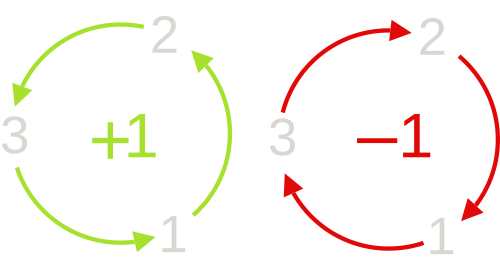
\includegraphics[width=0.5\linewidth]{Section/Figures/levi-civita-cycle-permutation.png}
    \caption{Levi-Civita Even and Odd Permutations}
\end{figure}

For example,
\begin{align*}
    \varepsilon_{123} &= 1 \\
    \varepsilon_{231} &= 1 \\
    \varepsilon_{312} &= 1 \\
    \varepsilon_{132} &= -1 \\
    \varepsilon_{213} &= -1 \\
    \varepsilon_{321} &= -1 \\
    \varepsilon_{122} &= 0 \\
    \varepsilon_{113} &= 0 \\
    \varepsilon_{111} &= 0 \\
\end{align*}

Since this is a third order tensor, there are 27 components. From these, 3 of these components are $+1$, 3 are $-1$, and 21 are $0$.

\subsubsection{Properties (in 3D)}
\begin{itemize}
    \item $\varepsilon_{ijk} = \varepsilon_{jki} = \varepsilon_{kij}$
    \item $\varepsilon_{ijk}\varepsilon_{ijk} = 6$
    \item $\varepsilon_{ijk}\varepsilon_{imn} = \delta_{jm}\delta_{kn} - \delta_{jn}\delta_{km}$
    \item $\varepsilon_{ijk} = -\varepsilon_{ikj}$
    \item $a_{ij}\varepsilon_{ijk} = \varepsilon_{ijk}a_{ij}$
\end{itemize}

\subsection{Vector and Tensor Operations}
\subsubsection{Multiplication of a Vector by a Scalar}
\begin{align*}
    \alpha \vec{A} &= \vec{B} \\
    \alpha A_i &= B_i
\end{align*}

\subsubsection{Dot Product of Two Vectors}
\begin{align*}
    \vec{A} \cdot \vec{B} &= C \\
    A_i B_i &= C
\end{align*}

\subsubsection{Cross Product of Two Vectors}
\begin{align*}
    \vec{A} \cross \vec{B} &= \vec{C} \\
    \varepsilon_{ijk}A_jB_k &= C_i 
\end{align*}

\subsubsection{Dot Product of Two Tensors (Tensor Product)}
\begin{align*}
    %use \otimes
    A \otimes B &= A_{ij}B_{jk}= C_{ik}
\end{align*}

\subsubsection{Double Dot Product of Two Tensors}
\begin{align*}
    A : B &= A_{ij}B_{ij} = C
\end{align*}
A property of the double dot product is that it is commutative, 
\begin{align*}
    A : B &= B : A
\end{align*}

\subsubsection{Nabla Operator}
The Nabla operator is a vector differential operator. It is defined as:
\begin{align*}
    \nabla &= \frac{\partial}{\partial x_i} = \partial_{i} 
\end{align*}
In vector notation,
\begin{align*}
    \nabla &= \begin{bmatrix}
        \frac{\partial}{\partial x_1} \\
        \frac{\partial}{\partial x_2} \\
        \frac{\partial}{\partial x_3}
    \end{bmatrix}
\end{align*}

\subsubsubsection{Gradient of a Scalar}
The gradient of a scalar is a vector. It is defined as:
\begin{align*}
    \nabla T &= \frac{\partial T}{\partial x_i} = \partial_{i} T
\end{align*}

\subsubsubsection{Gradient of a Vector}
The gradient of a vector is a tensor. It is defined as:
\begin{align*}
    \nabla \vec{A} &= \frac{\partial A_j}{\partial x_i} = \partial_{i} A_j \\
    &= \begin{bmatrix}
        \partial_{1} A_1 & \partial_{1} A_2 & \partial_{1} A_3 \\
        \partial_{2} A_1 & \partial_{2} A_2 & \partial_{2} A_3 \\
        \partial_{3} A_1 & \partial_{3} A_2 & \partial_{3} A_3
    \end{bmatrix}
\end{align*}

\subsubsubsection{Divergence of a Vector}
The divergence of a vector is a scalar. It is defined as:
\begin{align*}
    \nabla \cdot \vec{A} &= \frac{\partial A_i}{\partial x_i} = \partial_{i} A_i = \Div(\vec{A}) \\
    &= \partial_{1} A_1 + \partial_{2} A_2 + \partial_{3} A_3 \\
    &= C
\end{align*}

\subsubsubsection{Divergence of a Tensor}
The divergence of a rank 2 tensor is a vector. It is defined as:
\begin{align*}
    \nabla \cdot A &= \frac{\partial A_{ij}}{\partial x_i} = \partial_{i} A_{ij} \\
    &= \begin{bmatrix}
        \partial_{1} A_{11} + \partial_{2} A_{21} + \partial_{3} A_{31} \\
        \partial_{1} A_{12} + \partial_{2} A_{22} + \partial_{3} A_{32} \\
        \partial_{1} A_{13} + \partial_{2} A_{23} + \partial_{3} A_{33}
    \end{bmatrix}
\end{align*}

\subsubsubsection{Curl of a Vector}
The curl of a vector is a vector. It is defined as:
\begin{align*}
    \nabla \cross \vec{A} &= \varepsilon_{ijk}\partial_{j} A_k = \Curl(\vec{A}) \\
    &= \begin{bmatrix}
        \partial_{2} A_3 - \partial_{3} A_2 \\
        \partial_{3} A_1 - \partial_{1} A_3 \\
        \partial_{1} A_2 - \partial_{2} A_1
    \end{bmatrix}
\end{align*}

\subsubsubsection{Laplace of a Scalar}
The Laplace of a scalar is a scalar. It is defined as:
\begin{align*}
    \nabla^2 \phi &= \Div(\Grad(\phi)) = \nabla \cdot (\nabla \phi) \\
    &= \partial_{i} (\partial_{i} \phi)  = \partial_{i} \partial_{i} \phi \\
    &= \partial_{1} \partial_{1} \phi + \partial_{2} \partial_{2} \phi + \partial_{3} \partial_{3} \phi
\end{align*}

\subsubsubsection{Laplace of a Vector}
The Laplace of a vector is a vector. It is defined as:
\begin{align*}
    \nabla^2 \vec{A} &= \Div(\Grad(\vec{A})) = \nabla \cdot (\nabla \vec{A}) \\
    &= \partial_{i} (\partial_{i} A_j)  = \partial_{i} \partial_{i} A_j \\
    &= \begin{bmatrix}
        \partial_{1} \partial_{1} A_1 + \partial_{2} \partial_{2} A_1 + \partial_{3} \partial_{3} A_1 \\
        \partial_{1} \partial_{1} A_2 + \partial_{2} \partial_{2} A_2 + \partial_{3} \partial_{3} A_2 \\
        \partial_{1} \partial_{1} A_3 + \partial_{2} \partial_{2} A_3 + \partial_{3} \partial_{3} A_3
    \end{bmatrix}
\end{align*}

\subsubsubsection{Vector Outer Product (Dyadic Product)}
The vector outer product is a rank 2 tensor. It is defined as:
\begin{align*}
    \vec{A} \vec{B} &= \vec{A} \vec{B}^T  = \begin{bmatrix} a_1 \\ a_2 \\ a_3 \end{bmatrix} [b_1 \quad b_2 \quad b_3] \\
    &= \begin{bmatrix}
        a_1 b_1 & a_1 b_2 & a_1 b_3 \\
        a_2 b_1 & a_2 b_2 & a_2 b_3 \\
        a_3 b_1 & a_3 b_2 & a_3 b_3
    \end{bmatrix} \\
    &= A_i B_j = C_{ij}
\end{align*}

\subsection{Summary of Tensor Operations}
\begin{table}[H]
    \centering
    \caption{Summary of Tensor Operations}
    \begin{tabular}{p{0.5 \textwidth}cc}
        \toprule
        Description & Vector Notation & Einstein Notation \\
        \midrule
        Multiplication of a Vector by a Scalar & $\alpha \vec{A}$ & $\alpha A_i$ \\
        Dot Product of Two Vectors & $\vec{A} \cdot \vec{B}$ & $A_i B_i$ \\
        Cross Product of Two Vectors & $\vec{A} \cross \vec{B}$ & $\varepsilon_{ijk}A_jB_k$ \\
        Dot Product of Two Tensors (Tensor Product) & $A \otimes B$ & $A_{ij}B_{jk}= C_{ik}$ \\
        Double Dot Product of Two Tensors & $A : B$ & $A_{ij}B_{ij} = C$ \\
        Gradient of a Scalar & $\nabla T$ & $\partial_{i} T$ \\
        Gradient of a Vector & $\nabla \vec{A}$ & $\partial_{i} A_j$ \\
        Divergence of a Vector & $\nabla \cdot \vec{A}$ & $\partial_{i} A_i$ \\
        Divergence of a Tensor & $\nabla \cdot A$ & $\partial_{i} A_{ij}$ \\
        Curl of a Vector & $\nabla \cross \vec{A}$ & $\varepsilon_{ijk}\partial_{j} A_k$ \\
        Laplace of a Scalar & $\nabla^2 \phi$ & $\partial_{i} \partial_{i} \phi$ \\
        Laplace of a Vector & $\nabla^2 \vec{A}$ & $\partial_{i} \partial_{i} A_j$ \\
        Vector Outer Product (Dyadic Product) & $\vec{A} \vec{B}$ & $A_i B_j = C_{ij}$ \\
        \bottomrule
    \end{tabular}
\end{table}

\section{Flow Descriptions}
\subsection{Continuity Equation}
The continuity equation is a statement of the conservation of mass. The general form is given by:
\begin{align*}
    \frac{\partial \rho}{\partial t} + \nabla \cdot (\rho \vec{u}) &= 0  \\
    \underbrace{\frac{\partial \rho}{\partial t} + \vec{u} \cdot \nabla \rho}_{\frac{D\rho}{Dt}} + \rho \nabla \cdot \vec{u} &= 0
\end{align*}
where $D/Dt$ is the material derivative,
\begin{align*}
    \frac{D}{Dt} &= \frac{\partial}{\partial t} + \vec{u} \cdot \nabla
\end{align*}

\subsection{Momentum Equation}
The momentum equation is a statement of the conservation of momentum. There are many, many forms. The one most useful for this course is:
\begin{empheq}[box=\fbox]{align}
    \frac{\partial}{\partial t}(\rho v_i) + \frac{\partial}{\partial x_j}(\rho v_j v_i) &= -\frac{\partial p}{\partial x_i} + \frac{\partial}{\partial x_j}\left[\mu \left(\frac{\partial v_i}{\partial x_j} + \frac{\partial v_j}{\partial x_i}\right)\right] - \frac{\partial}{\partial x_i} \left[\frac{2}{3} \mu \frac{\partial v_k}{\partial x_k}\right] + \rho b_i
\end{empheq}
In cartesian coordinates, first in the $x$ direction,
\begin{empheq}[box=\fbox]{align}
    \frac{\partial}{\partial t}(\rho u) + \frac{\partial}{\partial x}(\rho u^2) + \frac{\partial}{\partial y}(\rho uv) + \frac{\partial}{\partial z}(\rho uw) &= -\frac{\partial p}{\partial x} + \frac{\partial}{\partial x}\left[\mu \left(\frac{\partial u}{\partial x} + \frac{\partial u}{\partial x}\right)\right] \\
    & \quad + \frac{\partial}{\partial y}\left[\mu \left(\frac{\partial u}{\partial y} + \frac{\partial v}{\partial x}\right)\right] + \frac{\partial}{\partial z}\left[\mu \left(\frac{\partial u}{\partial z} + \frac{\partial w}{\partial x}\right)\right] \nonumber \\
    & \quad - \frac{\partial}{\partial x} \left[\frac{2}{3} \mu \left(\frac{\partial u}{\partial x} + \frac{\partial v}{\partial y} + \frac{\partial w}{\partial z}\right)\right] + \rho b_x \nonumber
\end{empheq}
Then in the $y$ direction,
\begin{empheq}[box=\fbox]{align}
    \frac{\partial}{\partial t}(\rho v) + \frac{\partial}{\partial x}(\rho uv) + \frac{\partial}{\partial y}(\rho v^2) + \frac{\partial}{\partial z}(\rho vw) &= -\frac{\partial p}{\partial y} + \frac{\partial}{\partial x}\left[\mu \left(\frac{\partial v}{\partial x} + \frac{\partial u}{\partial y}\right)\right] \\
    & \quad + \frac{\partial}{\partial y}\left[\mu \left(\frac{\partial v}{\partial y} + \frac{\partial v}{\partial y}\right)\right] + \frac{\partial}{\partial z}\left[\mu \left(\frac{\partial v}{\partial z} + \frac{\partial w}{\partial y}\right)\right] \nonumber \\
    & \quad - \frac{\partial}{\partial y} \left[\frac{2}{3} \mu \left(\frac{\partial u}{\partial x} + \frac{\partial v}{\partial y} + \frac{\partial w}{\partial z}\right)\right] + \rho b_y \nonumber
\end{empheq}
Finally in the $z$ direction,
\begin{empheq}[box=\fbox]{align}
    \frac{\partial}{\partial t}(\rho w) + \frac{\partial}{\partial x}(\rho uw) + \frac{\partial}{\partial y}(\rho vw) + \frac{\partial}{\partial z}(\rho w^2) &= -\frac{\partial p}{\partial z} + \frac{\partial}{\partial x}\left[\mu \left(\frac{\partial w}{\partial x} + \frac{\partial u}{\partial z}\right)\right] \\
    & \quad + \frac{\partial}{\partial y}\left[\mu \left(\frac{\partial w}{\partial y} + \frac{\partial v}{\partial z}\right)\right] + \frac{\partial}{\partial z}\left[\mu \left(\frac{\partial w}{\partial z} + \frac{\partial w}{\partial z}\right)\right] \nonumber \\
    & \quad - \frac{\partial}{\partial z} \left[\frac{2}{3} \mu \left(\frac{\partial u}{\partial x} + \frac{\partial v}{\partial y} + \frac{\partial w}{\partial z}\right)\right] + \rho b_z \nonumber
\end{empheq}

\subsection{Energy Equation}
The general internal energy equation is too annoying to write out and isn't particularly useful. The one most useful for this course is the incompressible Newtonian fluid energy equation: 
\begin{empheq}[box=\fbox]{align}
    \rho C_p \left(\frac{\partial T}{\partial t} + \vec{u} \cdot \nabla T\right) &= k \nabla^2 T + \mu \left[2\left(\frac{\partial u}{\partial x}\right)^2 + 2\left(\frac{\partial v}{\partial y}\right)^2 + 2\left(\frac{\partial w}{\partial z}\right)^2 \right. \\
    & \quad + \left. \left(\frac{\partial u}{\partial y} + \frac{\partial v}{\partial x}\right)^2 + \left(\frac{\partial u}{\partial z} + \frac{\partial w}{\partial x}\right)^2 + \left(\frac{\partial v}{\partial z} + \frac{\partial w}{\partial y}\right)^2\right] \nonumber
\end{empheq}

\subsection{Common Simplifications}
Here are some common simplifications that are often made to the momentum and energy equations:
\begin{table}[H]
    \centering
    \caption{Common Simplifications}
    \begin{tabular}{p{0.5 \textwidth}cc}
        \toprule
        Description & Consequece \\
        \midrule
        Incompressible Flow & $\rho = \text{constant}$ \\
        Newtonian Fluid & $\mu = \text{constant}$ \\
        Steady Flow & $\frac{\partial}{\partial t} = 0$ \\
        2D Flow & $\frac{\partial \vec{u}}{\partial z} = 0$, $w = 0$ \\
        Fully Developed Flow & $\frac{\partial \vec{u}}{\partial x} = 0$ \\
        Gravity & $\vec{b} = -g \hat{k}$ \\
        Constant Pressure & $p = \text{constant}$ \\
        \bottomrule
    \end{tabular}
\end{table}
\section{Discretization Methods}

\subsection{Finite Volume Method}
Basically, take a differential equation and integrate it over a control volume. This gives us a discrete form of the equation.
\begin{figure}[H]
    \centering
    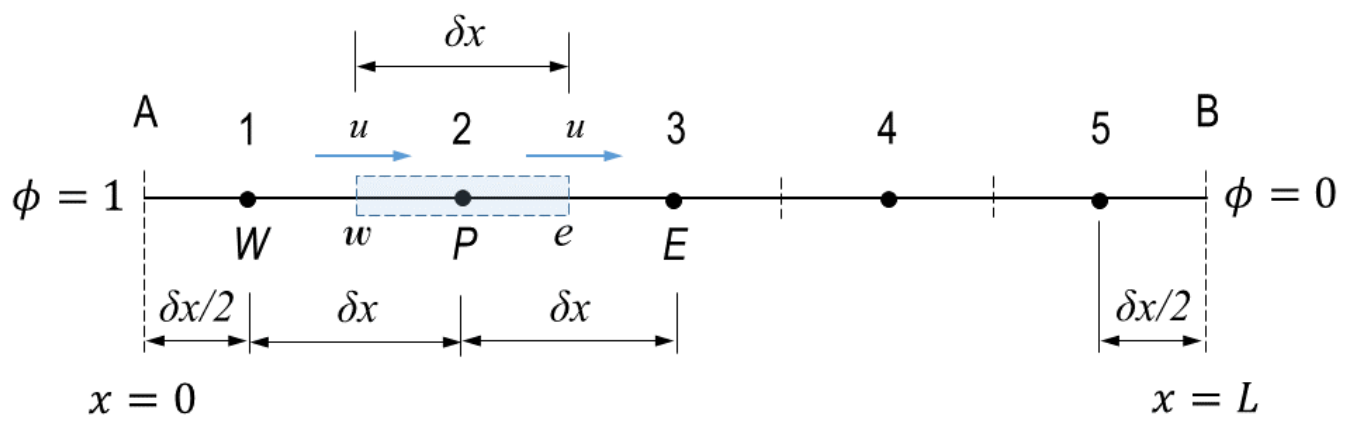
\includegraphics[width=0.8\textwidth]{Section/Figures/mesh generation.png}
    \caption{Grid generation for finite volume method}
\end{figure}
Consider the diffusion-convection equation with no source term:
\begin{align*}
    \frac{d}{dx} (\rho \vec{u} \phi) = \frac{d}{dx} (\Gamma \frac{d\phi}{dx})
\end{align*}
Integrating over the control volume:
\begin{align*}
    \int_{\text{CV}} \frac{d}{dx} (\rho \vec{u} \phi) dV &= \int_{\text{CV}} \frac{d}{dx} (\Gamma \frac{d\phi}{dx}) dV \\
    \int_{\Delta x} \frac{d}{dx} (\rho \vec{u} \phi) S dx &= \int_{\Delta x} \frac{d}{dx} (\Gamma \frac{d\phi}{dx}) S dx \\
    \left[ \rho \vec{u} \phi \right]_{w}^{e} &= \left[ \Gamma \frac{d\phi}{dx} \right]_{w}^{e} \\
    [\rho \vec{u} \phi]_{e} - [\rho \vec{u} \phi]_{w} &= \left[\Gamma \frac{d\phi}{dx} \right]_{e} - \left[\Gamma \frac{d\phi}{dx} \right]_{w} 
\end{align*}

\subsubsection{Central Difference Scheme}
The derivative terms can be approximated using the central difference scheme. 
\begin{empheq}[box=\fbox]{align}
    \frac{d\phi}{dx}_e & = \frac{\phi_E - \phi_P}{\Delta x_{PE}} \\
    \frac{d\phi}{dx}_w & = \frac{\phi_P - \phi_W}{\Delta x_{WP}}
\end{empheq}
For $\phi$ at the non-node points, the central difference scheme calculates the values of $\phi$ at $e$ and $w$ using linear interpolation:
\begin{empheq}[box=\fbox]{align}
    \phi_e & = \frac{\phi_P + \phi_E}{2} \\
    \phi_w & = \frac{\phi_P + \phi_W}{2}
\end{empheq}
And at Node 1 ($\phi_{W} = \phi_{A}$),
\begin{empheq}[box=\fbox]{align}
    \frac{d\phi}{dx}_w & = \frac{\phi_P - \phi_A}{\Delta x_{AP}} \\
    \phi_w & = \phi_A
\end{empheq}
And at Node N ($\phi_{E} = \phi_{B}$),
\begin{empheq}[box=\fbox]{align}
    \frac{d\phi}{dx}_e & = \frac{\phi_B - \phi_P}{\Delta x_{PB}} \\
    \phi_e & = \phi_B
\end{empheq}

Substituting these values into the finite volume equation:
\begin{align*}
    \rho \vec{u} \frac{\phi_E - \phi_P}{\Delta x_{PE}} - \rho \vec{u} \frac{\phi_P - \phi_W}{\Delta x_{WP}} &= \Gamma \frac{\phi_E - \phi_P}{\Delta x_{PE}} - \Gamma \frac{\phi_P - \phi_W}{\Delta x_{WP}} 
\end{align*} 
And then you can write it in the form
\begin{align*}
    a_P \phi_P = a_W \phi_W + a_E \phi_E + q
\end{align*}

\subsubsection{Upwind Scheme}
For flow in positive direction (W to E), the upwind scheme calculates the values of $\phi_{e}$ and $\phi_{w}$ using:
\begin{empheq}[box=\fbox]{align}
    \phi_e & = \phi_P \\
    \phi_w & = \phi_W
\end{empheq}
And in the negative direction (E to W), the upwind scheme calculates the values of $\phi_{e}$ and $\phi_{w}$ using:
\begin{empheq}[box=\fbox]{align}
    \phi_e & = \phi_E \\
    \phi_w & = \phi_P
\end{empheq}
The central difference scheme is used to evaluate the derivative terms.






% \section*{Conservation of Energy (Scalar)}

Energy is a scalar quantity, and therefore it can be identified \& formulated through the conservation of a scalar quantity:

Let's try $\phi = $ scalar,
\begin{align*}
    \frac{\partial}{\partial t} \int_{\text{C.V.}} \rho \phi \, dV 
    + \int_{\text{C.S.}} \rho \phi (\vec{u} \cdot \vec{n}) \, dS &= 
    \oint_{\text{C.S.}} \Gamma \Grad(\phi) \cdot \vec{n} \, dS + 
    \int_{\text{C.V.}} \underbrace{q_{\phi}}_{\text{source/sink}} \, dV
\end{align*}

\begin{align*}
    \implies 
    \frac{\partial}{\partial t} (\rho \phi)  
    + \frac{\partial}{\partial x_j} (\rho \phi u_j) &=
    \frac{\partial}{\partial x_j} (\Gamma \frac{\partial \phi}{\partial x_j}) + q_{\phi}
\end{align*}
Conservation of a scalar (Energy). In vector notation,
\begin{align*}
    \partial_{t} (\rho \phi) + \Div (\rho \phi \vec{u}) &= 
    \Div (\Gamma \Grad (\phi)) + q_{\phi} 
\end{align*}
Where
\begin{itemize}
    \item $\partial_{t} (\rho \phi)$ is the time rate of change of the scalar quantity $\phi$ (conservative term).
    \item $\Div (\rho \phi \vec{u})$ is the rate of change due to the flow due to $\vec{u}$ (advection term).
    \item $\Div (\Gamma \Grad (\phi))$ is the rate of change due to diffusion ($\Gamma$) (diffusion term).
    \item $q_{\phi}$ is the rate of production (source) or destruction (sink) of $\phi$.
\end{itemize}

\section*{Chapter 4. Fundamental flows (Simplification)}
Navier-Stokes equations are highly non-linear PDEs with no exact solutions. However,
there are fundamental flow dynamics (simplified flows) based on assumptions and approximations that 
makes the mathematics easier to follow, solve, and interpret.

We are going to look at 4 simplified flow cases:
\begin{enumerate}
    \item Incompressible flow ($\rho = \text{constant}$)
    \item Invicid flow (Euler's flow) ($\mu \to 0$)
    \item Creeping flow (Stokes flow) ($\text{Re} \ll 100$, inertial forces are negligible)
    \item Potential flow ($\text{Re} \to 0$, $\text{Ma} \to 0$
\end{enumerate}
Let's look at the conservation laws for each:
\subsection*{Incompressible flow}
Incompressibility is defined as incapability of a fluid (i.e. liquid) to compress to a smaller size
under internal/external loads. This, therefore, means that their \textbf{density $\rho$} does
not change as long as we keep their mass the same.

Typically, liquids are incompressible, but air (gas) can become compressible at special conditions.
\[
 \underbrace{\text{Ma}}_{\vec{u} /\text{speed of sound}} > 0.3 \implies \text{compressible}
\]

Continuity:
\begin{align*}
    \cancelto{0 (\text{Incomp})}{\frac{\partial \rho}{\partial t}} + \divergence (\rho \vec{u}) &= 0 \\
    \implies \divergence \vec{u} &= 0
\end{align*}
Momentum:
\begin{align*}
    \frac{\partial}{\partial t} (\rho \vec{u}) + \divergence (\rho \vec{u} \vec{u}) &=
    - \grad P + \cancelto{0, \;\text{continuity}}{\frac{1}{3} \mu \nabla(\divergence \vec{u})} + \mu \laplacian \vec{u} + \rho \vec{b} \\
\end{align*}
Expanding the $\divergence (\rho \vec{u} \vec{u})$ term,
\begin{align*}
    \divergence (\rho \vec{u} \vec{u}) &= (\divergence \rho \vec{u}) \vec{u}
        + \rho \vec{u} \cdot \grad \vec{u} \\
    &= \cancelto{0, \;\text{continuity}}{(\divergence \rho \vec{u})} \vec{u}
        + \rho \vec{u} \cdot \grad \vec{u} \\
    &= \rho \vec{u} \cdot \grad \vec{u}
\end{align*}
Therefore,
\begin{align*}
    \frac{\partial}{\partial t} (\rho \vec{u}) + \rho \vec{u} \cdot \grad \vec{u} &=
    - \grad P + \mu \laplacian \vec{u} + \rho \vec{b} \\
    \rho \frac{\partial \vec{u}}{\partial t} + \rho \vec{u} \cdot \grad \vec{u} &=
    - \grad P + \mu \laplacian \vec{u} + \rho \vec{b} \\
    \frac{\partial \vec{u}}{\partial t} + \vec{u} \cdot \grad \vec{u} &=
    -\frac{\grad P}{\rho} + \underbrace{\frac{\mu}{\rho}}_{\nu} \laplacian \vec{u} + \vec{b} \\
\end{align*}

\subsection*{Invicid flow (Euler's flow)}
Viscous forces can be important in flows close to a wall, where we have large velocity gradients (Also in wakes).
As we should before, it is the combination of $\nu$ and $\vec{u}$ that forms the viscous effects in transport of fluids. 

$\implies$ Vorticies $\to$ $\nu$ may be important.

$\hookrightarrow$ if you are far from a surface or regions of large velocity gradients, the implication of viscocity becomes minimal.

$\hookrightarrow$ we quantify the effect of viscocity in the flow using Reynold's Number:
\begin{align*}
    \text{Re} = \frac{\rho u \overbrace{L}^{\text{characteristic length}}}{\mu} 
    = \frac{\text{inertial forces}}{\text{viscous forces}}
\end{align*}
if Re $\gg 1000 \implies \mu \to 0$ which means inertial forces dominate the flow 
(negligible viscous forces).

Continuity:
\begin{align*}
    \frac{\partial \rho}{\partial t} + \divergence (\rho \vec{u}) &= 0 
\end{align*}
No impact because no $\mu$ term.

Momentum:
\begin{align*}
    \frac{\partial}{\partial t} (\rho \vec{u}) + \divergence (\rho \vec{u} \vec{u}) &=
    - \grad P + \cancelto{0, \;\text{invicid}}{\frac{1}{3}\mu \nabla(\divergence \vec{u})}
    + \cancelto{}{\mu \laplacian \vec{u}} + \rho \vec{b} \\
\end{align*}
\begin{align*}
    \boxed{\frac{\partial}{\partial t} (\rho \vec{u}) + \divergence (\rho \vec{u} \vec{u}) =
    - \grad P + \rho \vec{b}}
\end{align*}
Note: As we saw in the Navier-Stokes equation, the flow can only be dominated by the 
\textbf{Pressure} and \textbf{External forces}. This means that the invicid cond. cannot hold if we 
are dealing with areas of high straining (vorcity and wakes).

Note: Since we are assuring invicid condition, then the flow cannot slow down close to the 
stationary wall. $\implies$ Slip Boundary Condition.

\subsection*{Creeping flow (Stokes flow)}
At high re, we just discussed that viscous effects are negligible. Contrarily, at low 
Re, (Re $\ll 100$) the effect of viscosity \textbf{dominates} the flow. 

$\implies$ Inertial forces are negligible.

\begin{align*}
    \text{Re} \propto \frac{u D}{\nu} 
    \begin{cases}
        \text{Either } u \to 0 \text{and/or} \\
        D \to 0 
    \end{cases}
\end{align*}

Continuity:
\begin{align*}
    \frac{\partial \rho}{\partial t} + \divergence (\rho \vec{u}) &= 0
\end{align*}
No impact.

Momentum:
\begin{align*}
    0 = - \frac{\grad P}{\rho} +  \divergence (\nu \grad \vec{u}) + \vec{b} + \vec{b}
\end{align*}
This type of flow is mostly for porous media coating, or nano-fluidics.

\subsection*{Potential flow}
One of the simpliest flows in fluid mechanics.

Based on two conditions:
\begin{enumerate}
    \item Invicid flow ($\mu \to 0$)
    \item Irrotational flow ($\vec{\omega} \to 0$)
\end{enumerate}
provides approximation for initial flow conditions.
% \section*{Chapter 5: Non-Dimentionalization of the Flow}
Physically and mathematically, the flow results (dynamics) should not change based on the size of a simulation setup.

$\hookrightarrow$ Most fluid dynamics analyses are completed in a dimensionless framework. This allows for scaling of the real problem. 

$\hookrightarrow$ If the scaled conditions are maintained (i.e. Reynold's Number is the same), CFD simulations should be independent from geometrical or scalable physical parameters.

Note: The scalability of the flow condition holds only if the main flow behavior/dynamics is the same in terms of Re, $\rho$, $\mu$, \dots

Now, we return to our governing equations and discuss means to make them non-dimentionalized using normalization factors.

For example, velocity can be normalized using the freestream condition,
\begin{equation*}
    u_i = u_i^* u_{\infty} \implies u_i^* = \frac{u_i}{u_{\infty}}
\end{equation*}
where $u_{\infty}$ is the freestream velocity.

Similarly, 
\begin{equation*}
    t_0 = \frac{C}{u_{\infty}} \implies t^* = \frac{t}{t_0} = \frac{u_{\infty} t}{C}
\end{equation*}

For pressure,
\begin{equation*}
    P_{\text{dyn}} = \frac{1}{2} \rho u_{\infty}^2 \implies P^* = \frac{P}{P_{\text{dyn}}} = \frac{2 P}{\rho u_{\infty}^2}
\end{equation*}

and it is given that 
\begin{equation*}
    X_{i}^* = \frac{X_i}{C} \implies X_i = X_i^* C
\end{equation*}

$\hookrightarrow$ Now, let's begin with the continuity equation (incompressible)
\begin{align*}
    \frac{\partial u_i}{\partial x_i} &= 0 
\end{align*}
Substituting $u_i$ and $x_i$ with their non-dimensionalized counterparts,
\begin{align*}
    \frac{\partial u_i^* u_{\infty}}{\partial x_i^* C} &= 0 \\
    \cancel{\frac{u_{\infty}}{C}} \frac{\partial u_i^*}{\partial x_i^*} &= 0 \\
    \frac{\partial u_i^*}{\partial x_i^*} &= 0
\end{align*}

$\hookrightarrow$ Now, let's look at the momentum equation (incompressible)
\begin{align*}
    \frac{\partial u_i}{\partial t} + \frac{\partial (u_i u_j)}{\partial x_j} &= - \frac{1}{\rho} \frac{\partial P}{\partial x_i} + \nu \frac{\partial^2 u_i}{\partial x_j \partial x_j} + b_i
\end{align*}
Then,
\begin{align*}
    \frac{\partial (u_i^* u_{\infty})}{\partial (t^* t_0)} + \frac{\partial (u_i^* u_j^* u_{\infty}^2)}{\partial (x_j^* C)} 
    &= - \frac{1}{\rho} \frac{\partial (P^* P_{\text{dyn}})}{\partial (x_i^* C)} + \nu \frac{\partial^2 (u_i^* u_{\infty})}{\partial (x_j^* C) \partial (x_j^* C)} + g b_i^* \\
    \frac{\partial (u_i^* u_{\infty})}{\partial (t^* t_0)} + \frac{\partial (u_i^* u_j^* u_{\infty}^2)}{\partial (x_j^* C)}
    &= - \frac{1}{\rho} \frac{\partial (P^* P_{\text{dyn}})}{\partial (x_i^* C)} + \nu \frac{\partial^2 (u_i^* u_{\infty})}{\partial (x_j^* C) \partial (x_j^* C)} + g b_i^* \\
    \left(\frac{u_{\infty}}{t_0}\right) \frac{\partial u_i^*}{\partial t^*} + \left(\frac{u_{\infty}^2}{C}\right) \frac{\partial (u_i^* u_j^*)}{\partial x_j^*}
    &= - \frac{1}{\rho} \left(\frac{\frac{1}{2}\rho u_{\infty}^2}{C}\right) \frac{\partial P^*}{\partial x_i^*} + \left(\frac{\nu u_{\infty}}{C^2}\right) \frac{\partial^2 u_i^*}{\partial x_j^* \partial x_j^*} + g b_i^* 
\end{align*}
Now multiply by $C/u_{\infty}^2$,
\begin{align*}
    \frac{C}{u_\infty t_0}\frac{\partial u_i^*}{\partial t^*} + \frac{\partial (u_i^* u_j^*)}{\partial x_j^*}
    &= - \frac{1}{2} \frac{\partial P^*}{\partial x_i} + \frac{\nu}{u_{\infty} C} \frac{\partial^2 u_i^*}{(\partial x_j^*)^2} + \frac{g C}{u_{\infty}^2} b_i^*
\end{align*}
Therefore we obtain a number of important characteristic flow quantities:
\begin{enumerate}
    \item Strouhal Number: This dimentionless number is wkd as a number to describe flow unsteadiness (periodicity). Hence, $f_i = 1/t_i$ in the frequency of unsteadiness, which relates to vortex formulation frequency, flapping wings, etc.
    \begin{equation*}
        \text{St} = \frac{f_i C}{u_{\infty}} = \frac{C}{\underbrace{P_i}_{\text{Period}} u_{\infty}}
    \end{equation*}
    \item Reynold's Number: Describes the ratio of inertial to viscous effects.
    \begin{equation*}
        \text{Re} = \frac{\rho u_{\infty} C}{\mu} = \frac{u_{\infty} C}{\nu}
    \end{equation*}
    \item Froude Number: Describes the ratio of inertial to external fields in the flow
    \begin{equation*}
        \text{Fr} = \frac{u_{\infty}}{\sqrt{Cg}}
    \end{equation*}
    This enables us to understand if the flow is driven by inertial forces or external effects (gravity)
\end{enumerate}
From the energy equation, we will get the Peclet Number, which describes the ratio of convection to diffusion effects.
\begin{equation*}
    \text{Pe} = \frac{C u_{\infty}}{k/\rho C_p}
\end{equation*}


 %questions for after class
    %1. what happened to the time term in the inviscid continuity equation?
% \subsection*{Boundary Layer Approximation}
Boundary layers are one of the most common fluid flow phenomena observed in nature. In fact, the wind on an Earth's atmosphere is the result of a boundary layer developed by moving air next to the planet's surface. This is referred to as the atmospheric boundary.
$\hookrightarrow$ Correct understanding of the flow dynamics inside the boundary layer is critical in technology development, control systems, and weather forecasting. 

In classical fluid mechanics, we make unique assumptions, based in which we can apply certain approximating to our governing equations. For a laminar boundary layer, there are 3 assumption that drive our approximation process.
\begin{enumerate}
    \item B.L are 2-D. $\implies$ at high Re, this can become problematic.
    \item The thickness of the B.L. ($\delta$) is small compared to the other characteristic length. $\implies$ Mostly true.
    \item The flow velocity in the streamwise direction dominates. $\implies$ Provable.
\end{enumerate}
\begin{figure}
    \centering
    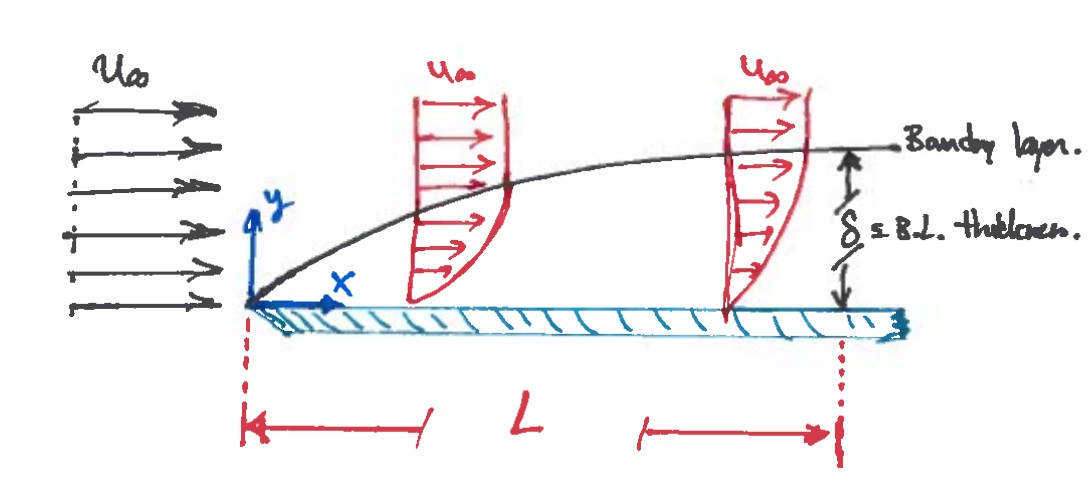
\includegraphics[width=0.5\linewidth]{Lecture Number/Figures/Lecture 6, Jan 30, 2024, Boundary Layer Concept.jpg}
    \caption{Boundary Layer Concept}
    \label{fig:Boundary Layer Concept}
\end{figure}
Assuming that Re$_{l} \gg 1$ and $\delta \ll \ell$, then we can rely on the following normalization factors (order of magnitude analysis).
\begin{table}
    \centering
    \caption{Order of Magnitude Analysis}
    \label{tab:Order of Magnitude Analysis}
    \begin{tabular}{c|ccc}
        & \textbf{Variable} & \textbf{Order of Magnitude} & \textbf{Normalization Factor} \\
        \hline
        Streamline Velocity & $u$ & $u_{\infty}$ & $u = u^* u_{\infty}$ \\
        Streamline Spatial Coordinate & $x$ & $\ell$ & $x = x^* \ell$ \\
        Orthogonal Directional Coordinate & $y$ & $\delta$ & $y = y* \delta$ \\
        Orthogonal Velocity & $v$ & $\mathcal{V}$?? & $v = v* \mathcal{V}$ \\
        \end{tabular}
\end{table}
Let's start with the continuity equation (incompressible flow):
\begin{gather*}
    \frac{\partial u_i}{\partial x_i} = 0 \\
    \frac{\partial u}{\partial x} + \frac{\partial v}{\partial y} = 0 \\
    \frac{\partial u^* u_{\infty}}{\partial x^* \ell} + \frac{\partial v^* \mathcal{V}}{\partial y^* \delta} = 0 \\
    \implies \left(\frac{u_{\infty}}{\ell}\right) \frac{\partial u^*}{\partial x^*} + \left(\frac{\mathcal{V}}{\delta}\right) \frac{\partial v^*}{\partial y^*} = 0 \\
    \implies \frac{\partial u^*}{\partial x^*} +\frac{\mathcal{V} \ell}{u_{\infty} \delta} \frac{\partial v^*}{\partial y^*} = 0 \\
\end{gather*}
Based on the order of magnitude analysis, 
\begin{gather*}
    \frac{\mathcal{V} \ell}{u_{\infty} \delta} = 1 \\
    \implies \mathcal{V} = \frac{u_{\infty} \delta}{\ell} \\
\end{gather*}
Therefore, if $\delta ll \ell$, then $\mathcal{V} \ll u_{\infty}$. This provies that streamline velocity dominates. 

Now, let's move to the Navier-Stokes equation. First, the x-dir:
\begin{gather*}
    \cancelto{\frac{\partial u}{\partial t}}{\text{S.S.}} + u \frac{\partial u}{\partial x} + v \frac{\partial u}{\partial y} = -\frac{1}{\rho} \frac{\partial P}{\partial x} + \nu \left(\frac{\partial^2 u}{\partial x^2} + \frac{\partial^2 u}{\partial y^2}\right) 
\end{gather*}
y-dir:
\begin{gather*}
    \cancelto{\frac{\partial v}{\partial t}}{\text{S.S.}} + u \frac{\partial v}{\partial x} + v \frac{\partial v}{\partial y} = -\frac{1}{\rho} \frac{\partial P}{\partial y} + \nu \left(\frac{\partial^2 v}{\partial x^2} + \frac{\partial^2 v}{\partial y^2}\right)
\end{gather*}

Let's look at the x-dir expression:
\begin{gather*}
    (u^* u_{\infty}) \frac{\partial (u^* u_{\infty})}{\partial (x^* \ell)} + (v^* \mathcal{V}) \frac{\partial (u^* u_{\infty})}{\partial (y^* \delta)} = -\frac{1}{\rho} \frac{\partial P}{\partial (x^* \ell)} + \nu \left(\frac{\partial^2 (u^* u_{\infty})}{\partial (x^* \ell)^2} + \frac{\partial^2 (u^* u_{\infty})}{\partial (y^* \delta)^2}\right) \\
    %---------------------------------------
    \implies \left(\frac{u_{\infty}^2}{\ell}\right) u^* \frac{\partial u^*}{\partial x^*} + \left(\frac{u_{\infty} \mathcal{V}}{\delta}\right) v^* \frac{\partial u^*}{\partial y^*} = -\frac{1}{\rho \ell} \frac{\partial P}{\partial x^*} + \nu \left(\left(\frac{u_{\infty}}{\ell^2}\right) \left(\frac{\partial^2 u^*}{\partial (x^*)^2} + \left(\frac{u_{\infty}}{\delta^2}\right) \frac{\partial^2 u^*}{\partial (y^*)^2}\right)\right) 
\end{gather*}
Using $\mathcal{V} = \frac{u_{\infty} \delta}{\ell}$, 
\begin{gather*}
    \left(\frac{u_{\infty}^2}{\ell}\right) u^* \frac{\partial u^*}{\partial x^*} + \left(\frac{u_{\infty}^2}{\ell}\right) v^* \frac{\partial u^*}{\partial y^*} = -\frac{1}{\rho \ell} \frac{\partial P}{\partial x^*} + \frac{\nu u_{\infty}}{\delta^2} \left(\cancelto{\left(\frac{\delta^2}{\ell^2}\right)}{0} \frac{\partial^2 u^*}{\partial (x^*)^2} + \frac{\partial^2 u^*}{\partial (y^*)^2}\right) 
\end{gather*}
Note the term inside the $\nu$ term is zero since $\delta \ll \ell$. From order of magnitude analysis, we can say
\begin{equation*}
    \text{Scaling of LHS} ~ \text{Scaling of RHS}
\end{equation*}
% i missed this part
% \begin{gather*}
%     \frac{u_{\infty}^2}{\ell} \sim \frac
\begin{gather*}
    \frac{\delta^2}{\ell^2} ~ \frac{\nu}{\ell u_{\infty}} = \frac{1}{\text{Re}}
\end{gather*}
So, if $\delta^2 \ll \ell^2$, then $\frac{1}{\text{Re}} \ll 1$. This implies the flow remains 2D for high Re. 

At this point, we can look at the scaling for pressure,
\begin{gather*}
    \frac{u_{\infty}^2}{\ell} ~ (\text{Pressure Scaling}) \left(\frac{1}{\rho}
    \frac{\partial P}{\partial x} = 0 \left(\frac{\rho u_{\infty}^2}{\ell}\right)\right)
\end{gather*}
Let's apply the same process to the y-direction. The results are:
\begin{gather*}
    \left(\frac{u_{\infty} \mathcal{V}}{\ell}\right) u^* \frac{\partial v^*}{\partial x^*} + \left(\frac{\mathcal{V}^2}{\delta^2}\right) v^* \frac{\partial v^*}{\partial y^*} = -\frac{1}{\rho} \frac{\partial P}{\partial y} + \nu \left(\left(\frac{\mathcal{V}}{\ell^2}\right) \frac{\partial^2 v^*}{\partial (x^*)^2} + \left(\frac{\mathcal{V}}{\delta^2}\right) \frac{\partial^2 v^*}{\partial (y^*)^2}\right) 
\end{gather*}
Since $\delta/\ell \ll 1$ and $u_{\infty} \mathcal{V}/\ell = 0$
\begin{gather*}
    \implies 0 = \frac{1}{\rho} \frac{\partial P}{\partial y^*} 
\end{gather*}
We can see that 
\begin{gather*}
    \text{Scaling of } \frac{\partial P}{\partial y} ~ \frac{u_{\infty}^2 \delta}{\ell^2} \\
    % \frac{\partial P}{\partial x} ~ \rho \frac{\u_{\infty}^2}{\ell} 
\end{gather*}
We can again show that 
\begin{gather*}
    \frac{\partial P}{\partial x} gg \frac{\partial P}{\partial y} 
\end{gather*}
% \subsection*{Example}
Consider a viscous liquid in steady state that is in a downward motion in a narrow channel. 
\begin{figure}[h]
    \centering
    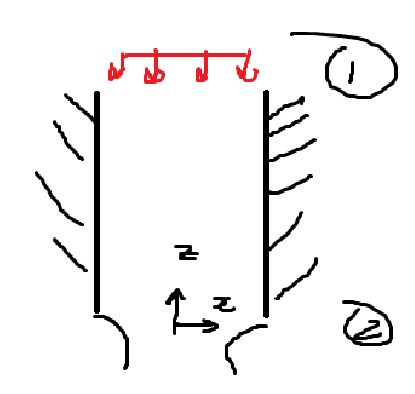
\includegraphics[width=0.2\textwidth]{Lecture Number/Figures/example 1, Feb 1, 2024.png}
    \caption{Viscous Liquid in a Narrow Channel}
    \label{fig:Example 1, Feb 1, 2024}
\end{figure}
\begin{enumerate}[label=(\alph*)]
    \item Write the full Navier-Stokes equations in the z-direction with body forces using index notation.
    \item Simplify the obtained equation from (a) for a fully-developed, 2D, steady flow with cartesian viscosity across the channel width. 
\end{enumerate}

(a) We write the general form of the Navier-Stokes equation:
\begin{align*}
    \frac{\partial}{\partial t} (\rho u_i) + \frac{\partial}{\partial x_j} (\rho u_i u_j) = -\frac{\partial P}{\partial x_i} + \frac{\partial}{\partial x_j} \left(\mu \left(\frac{\partial u_i}{\partial x_j} + \frac{\partial u_j}{\partial x_i}\right)\right) - \frac{\partial}{\partial x_i} \left(\frac{2}{3}\mu \frac{\partial u_k}{\partial x_k}\right) + \rho b_i
\end{align*}
in the z-dir, $i = 3$:
\begin{align*}
    \boxed{\partial_{t} (\rho w) + \partial_{j} (\rho w u_j) = -\partial_{z} P + \partial_{j} \left(\mu \left(\partial_{j} w + \partial_{i} u_j\right)\right) - \partial_{z} \left(\frac{2}{3}\mu \partial_{k} u_k\right) + \rho b_z}
\end{align*}
(b) We need to write out our assumptions and their approximations
\begin{table}[h]
    \centering
    \begin{tabular}{c|c}
        Assumption & Approximation \\
        \hline
        Viscous flow & No slip B.C. @ walls\\
        Incompressibe flow & $\rho = $ constant \\
        Steady State & $\partial_t = 0$ \\
        2D flow & $\partial_y = 0$ \\
        Fully developed & $\partial u_i/\partial x \gg \partial u_i/\partial z$ $\implies$ $\partial u_i / \partial z = 0$ \\
        \end{tabular}
\end{table}
Now, we can start applying the approximation to our governing equations. First, continuity,
\begin{gather*}
    \rho \cdot (\rho \vec{u}) = 0 \\
    \implies \partial_x u + \cancelto{\text{2D}}{\partial_y v} + \cancelto{\text{fully dev.}}{\partial_z w} = 0 \\
    \implies \partial_x u = 0 \\
    \implies u = c_1 
\end{gather*}
Since we have no-slip at the walls,
\begin{align*}
    u|_{x = \text{width}/2} = 0 \implies c_1 = 0
\end{align*}
Now, let's move to our z-direction Navier-Stokes equation:
\begin{align*}
    \cancelto{\text{S.S.}}{\partial_{t} (\rho w)} +\partial_{x} (\rho u  \cancelto{\text{cont.}} {w}) + \partial_{y} (\rho v \cancelto{\text{2D}}{w}) + \cancelto{\text{fully dev.}}{\partial_{z}} (\rho w^2) &= -\partial_{z} P + \partial_{x} \left(\mu \left(\partial_{x} \cancelto{\text{2D}}{w} + \cancelto{\text{fully dev.}}{\partial_{z} u}\right)\right) \\
    &+ \cancelto{\text{2D}}{\partial_{y}} \left(\mu \left(\partial_{y} w + \partial_{z} v\right)\right) + \partial_{z} \left(\mu \cancelto{\text{fully dev.}}{\left(\partial_{z} w + \partial_{z} w\right)}\right) \\
    &- \partial_{z} \left(\frac{2}{3}\mu \cancelto{\text{cont.}}{\left(\partial_{x} u + \partial_{y} v + \partial_{z} w\right)} \right)+ \rho b_z 
\end{align*}
Therefore,
\begin{gather*}
    0 = - \partial_{z} P + \partial_{x} \left(\mu \partial_x w\right) + \rho b_z \\
    \implies \partial_z P = \mu \partial_{xx} w + \rho b_z
\end{gather*}
At location (2), we have that flow open to outside. This means that the flow cannot be fully developed.
\begin{equation*}
    P_2 = P_{\text{atm}}
\end{equation*}
\begin{table}[h]
    \centering
    \begin{tabular}{c|c}
        Assumptions & Approximations \\
        \hline
        Incomp. flow & $\rho = \text{constant}$ $\implies \nabla \cdot \vec{u} = 0$ \\
        2D flow & $\partial_y = 0$  and $v = 0$ \\
        Steady State & $\partial_t = 0$ \\
        Open to air & $P_2 = P_{\text{atm}}$ \\
        Gravity & $b_z = -g$ \\
    \end{tabular}
\end{table}
\begin{align*}
    \cancelto{\text{S.S.}}{\partial_{t} (\rho w)} + \partial_{x} (\rho u w) + \cancelto{\text{2D}}{\partial_{y} (\rho v w)} + \partial_{z} (\rho w^2) &= -\cancelto{\text{Atm.}}{\partial_{z} P} + \partial_{x} \left(\mu \left(\partial_{x} w + \partial_{z} u\right)\right) \\
    &+ \partial_{y} \left(\mu \cancelto{\text{cont.}}{\left(\partial_{y} w + \partial_{z} v\right)} \right) + \partial_{z} \left(\mu \left(\partial_{z} w + \partial_{z} w\right)\right) \\
    &- \partial_{z} \left(\frac{2}{3}\mu \cancelto{\text{cont.}}{\left(\partial_{x} u + \partial_{y} v + \partial_{z} w\right)}\right)+ \rho b_z
\end{align*}
Which simplifies to 
\begin{align*}
    \partial_{x} (uw) + \partial_{z} (\rho w^2) &= \nu \partial_{x} \left(\partial_{x} w + \partial_{z} u\right) + \nu \partial_{z} \left(2\partial_{z} w\right) - g \\
    \implies w \partial_x u + u \partial_x w + 2 w \partial_z w &= \nu \left(\partial_{xx} w + \partial_{xz} u + 2 \partial_{zz} w\right) - g 
\end{align*}

Consider a heat conduction at steady state with no source or sink. The boundary conditions are:
\begin{align*}
    @ x = 0, \quad T = T_1 \\
    @ x = L, \quad T = T_2
\end{align*}
Now, solve for temperature distribution across the solid in a 1D case.
\begin{align*}
    \rho C_p \partial_t T + \rho C_p \partial_x^2 T &= k \partial_x^2 T
    + Q 
\end{align*}
Now assumptions,
\begin{table}[h]
    \centering
    \begin{tabular}{c|c}
        Assumptions & Approximations \\
        \hline
        Steady State & $\partial_t = 0$ \\
        No flow & $u = 0$ \\
        No source/sink & $Q = 0$ \\
        \end{tabular}
\end{table}
\begin{gather*}
    \implies 0 = k \partial_x^2 T \\
    T = c_1 x + c_2
\end{gather*}
Now, applying boundary conditions, 
\begin{align*}
    T|_{x = 0} = T_1 \implies c_2 = T_1 \\
    T|_{x = L} = T_2 \implies c_1 L + T_1 = T_2 \implies c_1 = \frac{T_2 - T_1}{L}
\end{align*}
Therefore,
\begin{equation*}
    T = \frac{T_2 - T_1}{L}x + T_1
\end{equation*}

\subsection*{Example 3}
Consider the example above but with the following changes
\begin{itemize}
    \item There is a constant heat source in the material
    \item The wall at $x = L$ is adiabatic ($\partial_x T = 0$) 
    \item The B.C at $x= 0 $ stays $T = T_1$
\end{itemize}   
\begin{align*}
    \cancelto{\text{S.S}}{\rho C_p \partial_t T} + \rho C_p \cancelto{\text{No flow}}{\partial_x u} \partial_x T &= k \partial_x^2 T + Q
\end{align*}
So,
\begin{align*}
    k \partial_x^2 T &= -Q \\
    \implies T &= \frac{-Q}{2k}x^2 + c_1 x + c_2
\end{align*}
Using the boundary conditions,
\begin{align*}
    T &= \frac{-Q}{2k}\left(\frac{x^2}{2} - Lx\right) + T_1
\end{align*}
% \newpage
% %\bibliographystyle{IEEEtran}
% %\bibliography{citations.bib}
% %\bibliography{}

% \newpage
% \appendix
% \section{Appendix: Arduino Uno Accuracy}
\label{sec:appendix-arduino-accuracy}
Table \ref{tab:arduino-accuracy-appendix} summarizes the range, resolution, repeatability, accuracy, and manufacturer's accuracy for various ranges of the 
Arduino Uno. Sample calculations for the 5V reference voltage are shown below. Note, the manufacturer's accuracy is $\pm$ 2 LSBs.

\begin{align*}
    \text{Resolution} &= \frac{V_{\text{ru}} - V_{\text{rl}}}{2^n} \\
    &= \frac{5.000 - 0.000}{2^{10}} \\
    &= \boxed{\qty[per-mode=symbol]{4.883}{\milli\volt\per\LSB}} \\
    \text{Repeatability} &= \max({\text{Max Deviation}}) \\
    &= \max(\langle 5.00, 0.00, 9.00, 44.00 \rangle) \\
    &= \boxed{\qty{44.00}{\milli\volt}} \\
    \text{Accuracy} &= \max({\text{Deviation}}) \\
    &= \max\left(
        \tiny	
        \begin{bmatrix}
            -0.009 & -0.009 & -0.009 & -0.009 & -0.009 & -0.009 & -0.009 & -0.009 & -0.004 & -0.009 \\
            0.001 & 0.001 & 0.001 & 0.001 & 0.001 & 0.001 & 0.001 & 0.001 & 0.001 & 0.001 \\
            0.016 & 0.021 & 0.012 & 0.016 & 0.012 & 0.012 & 0.016 & 0.016 & 0.012 & 0.016 \\
            0.02 & 0.024 & 0.02 & 0.024 & 0.01 & 0.02 & \textbf{0.054} & 0.024 & 0.034 & 0.02 \\
        \end{bmatrix}
    \right) \nonumber \\
    &= \boxed{\qty{54.00}{\milli\volt}}\\
    \text{Manuf. Acc.} &= \qty{2}{\LSB} \times \text{Resolution} \\
    &= \boxed{\qty{9.766}{\milli\volt}}
\end{align*}

\noindent For significant figures, since the range is given to 3 decimal places, the resolution is given to 3 decimal places, more often
than not, the number of significant figures is 4. This is because addition and subtraction do not take into account the number of significant figures
but rather the number of decimal places.

\begin{table}[ht]
    \caption{Range, Resolution, Repeatability, Accuracy, and Manufacturer's Accuracy for Various Ranges of the Arduino Uno}
    \label{tab:arduino-accuracy-appendix}
    \centering
    \small
    \begin{tabular}{lccccc}
        \toprule
        Arduino Config. & Range & Resolution & Repeatability & Acc. & Manuf. Acc. \\
        & (V) & (mV/LSB) & (mV) & (mV) & (mV) \\
        \midrule
        5V Ref. & 0.000 - 5.000 & 4.883 & 44.00 & 54.00 & 9.766 \\
        3.3V Ref. & 0.000 - 3.300 & 3.223 & 4.000 & 17.00 & 6.445 \\
        3.3V Ref., 10x VDiv & 0.00 - 33.00 & 32.23 & 32.00 & 83.00 & 64.45 \\
        3.3V Ref., [-10, 10]V & -10.00 - 10.00 & 19.53 & 0.000 & 24.00 & 39.06 \\
        3.3V Ref., 10x Amp. & 0.000 - 0.330 & 0.3223 & 0.000 & 0.000 & 0.6445 \\
        \bottomrule
    \end{tabular}
\end{table}

\FloatBarrier
\phantom{a}
\end{document}